\documentclass{beamer} 
\usepackage{amsmath,amsthm}
\usepackage{graphicx,microtype,parskip}
\usepackage{caption,subcaption,multirow}
\usepackage{attrib}

\frenchspacing

\usetheme{default}
\usecolortheme{whale}

\setbeamertemplate{navigation symbols}{}

\setbeamercolor{title}{fg=blue,bg=white}

\setbeamercolor{block title}{fg=white,bg=gray}
\setbeamercolor{block body}{fg=black,bg=lightgray}

\setbeamercolor{block title alerted}{fg=white,bg=darkgray}
\setbeamercolor{block body alerted}{fg=black,bg=lightgray}

\AtBeginSection[]
{
  \begin{frame}
    \tableofcontents[currentsection]
  \end{frame}
}

\title{}
\author{Peter D Smits}
\institute{Committee on Evolutionary Biology, University of Chicago}
\date{}

\begin{document}

\begin{frame}
  \tableofcontents
\end{frame}

\section{Since last meeting}
\begin{frame}
  \begin{block}{Since last meeting}
    \begin{itemize}
      \item Evolution 2015 talk
      \item GSA 2015 talk
      \item Chapter 1 published (PNAS)
        \begin{itemize}
          \item Effects of biotic traits on mammal species duration
        \end{itemize}
      \item Chapter 2 submitted (Evolution)
        \begin{itemize}
          \item Interplay between extinction intensity and selectivity in brachiopod extinction
          \item Submitted early October, still in review?
        \end{itemize}
      \item Did not submit DDIG
    \end{itemize}
  \end{block}
\end{frame}

\begin{frame}
  \frametitle{Review possible chapter 1}
  % Smits 2015 PNAS
  % i took all of your comments very seriously and they really improved the paper
  %   rick for forcing on the phylo (didn't do figure, but made make me use it)
  %   ken and david for pushing about modern extinction risk
  %   michael and ken for helping me write it in english
  % sorry i didn't send it to anyone except michael and ken
\end{frame}

\begin{frame}
  \frametitle{Review possible chapter 2}
  % Submitted to Evolution
  % what my patterns in Australia project eventually turned into
  %   sorry about that
  %   because length of record 
  %   also because model complexity and size of data needed
  % sorry i didn't send it to anyone except michael and ken
  %   this is actually a really good time to get all of your comments!
\end{frame}

\section{Current projects}
\subsection{Brachiopods}
\begin{frame}
  \frametitle{Regional patterns in the diversification of Paleozoic brachiopods}
  \begin{alertblock}{Question}
    How does differential taxonomic entrance and loss contribute to regional (e.g. latitudinal) diversity?
  \end{alertblock}
\end{frame}

\begin{frame}
  \begin{block}{Motivation}
    \begin{itemize}
      \item latitudinal diversity gradients
        \begin{itemize}
          \item through lense of a diversification process
        \end{itemize}
      \item regional as opposed to global
        \begin{itemize}
          \item variation within regions may not match global pattern \\(more biologically relevant?)
          \item partial follow up to brachiopod survival work
        \end{itemize}
    \end{itemize}
  \end{block}
\end{frame}

\begin{frame}
  \frametitle{Brachiopod latitudinal diversity}
  \begin{center}
    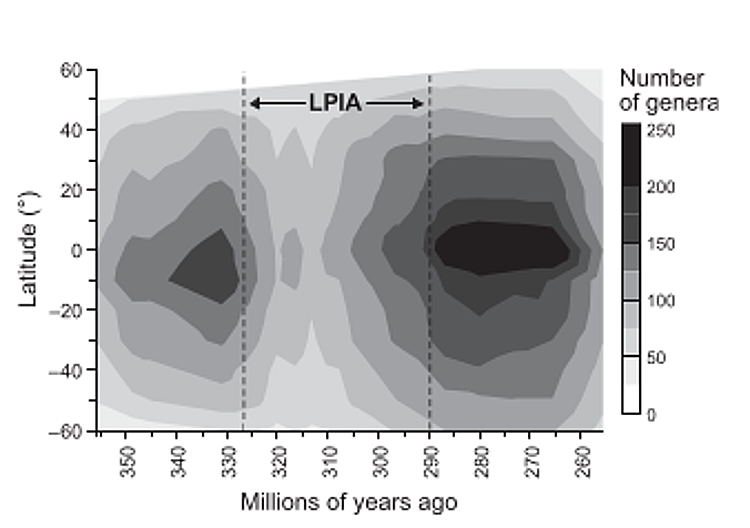
\includegraphics[width=\textwidth,height=0.8\textheight,keepaspectratio=true]{figure/powell_2007}
  \end{center}

  \attrib{\small{Powell 2007 \emph{G. Eco. Biogeo.}}}
\end{frame}

\begin{frame}
  \frametitle{Variation in bioversity gradient}
  \begin{columns}
    \begin{column}{0.4\textwidth}
      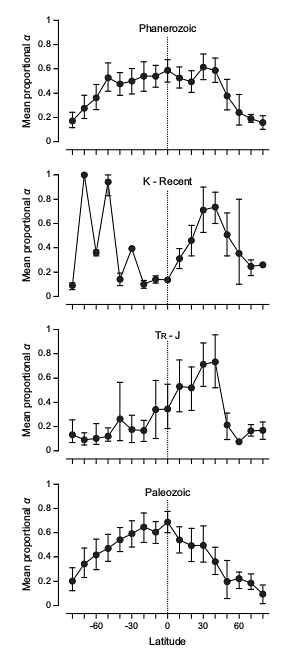
\includegraphics[width=\textwidth,height=0.8\textheight,keepaspectratio=true]{figure/powell_2015_b}
    \end{column}
    \begin{column}{0.6\textwidth}
      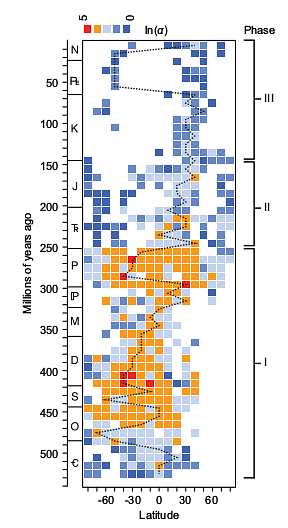
\includegraphics[width=\textwidth,height=0.7\textheight,keepaspectratio=true]{figure/powell_2015_a}
    \end{column}
  \end{columns}

  \attrib{\small{Powell \textit{et al} 2015 \emph{Paleobio.}}}
\end{frame}

\begin{frame}
  \frametitle{``Modes'' of latitudinal diversity}
  \begin{columns}
    \begin{column}{0.55\textwidth}
      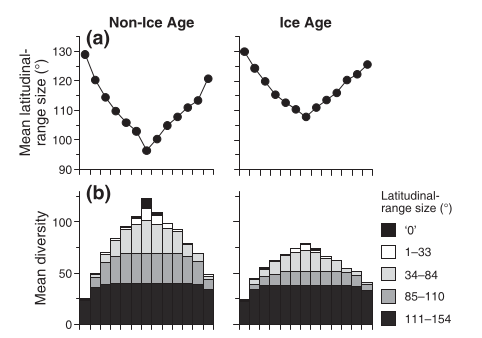
\includegraphics[width=\textwidth,height=0.8\textheight,keepaspectratio=true]{figure/powell_2007_a}
    \end{column}
    \begin{column}{0.5\textwidth}
      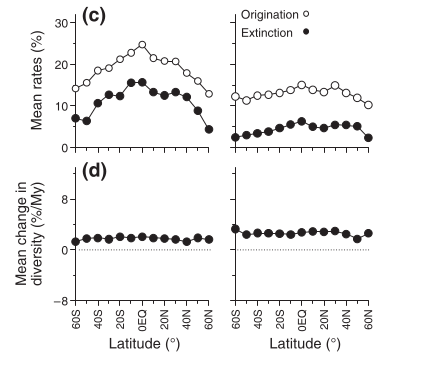
\includegraphics[width=\textwidth,height=0.8\textheight,keepaspectratio=true]{figure/powell_2007_b}
    \end{column}
  \end{columns}

  \attrib{\small{Powell 2007 \emph{G. Eco. Biogeo.}}}
\end{frame}

\begin{frame}
  \frametitle{Change in evenness + diversity}
  \begin{center}
    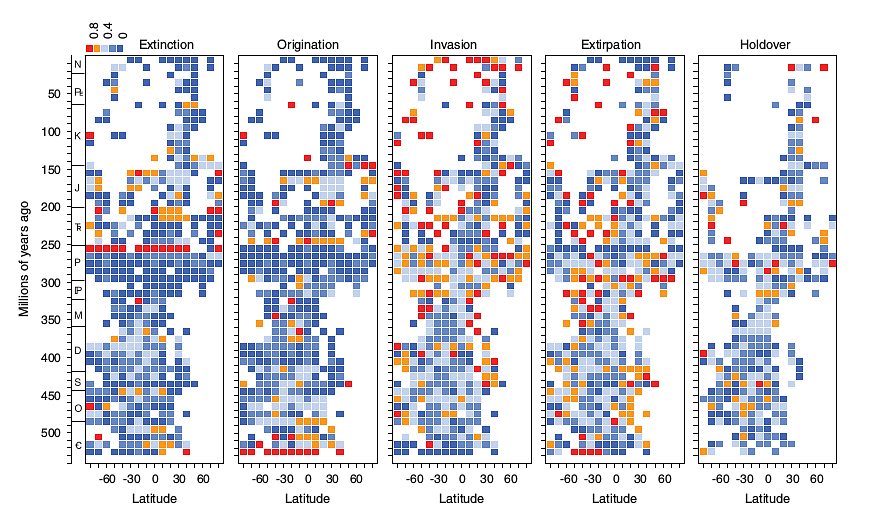
\includegraphics[width=\textwidth,height=0.8\textheight,keepaspectratio=true]{figure/powell_2015}
  \end{center}

  \attrib{\small{Powell \textit{et al} 2015 \emph{Paleobio.}}}
\end{frame}


\begin{frame}
  \frametitle{Model structure: Markov model}
  \begin{center}
    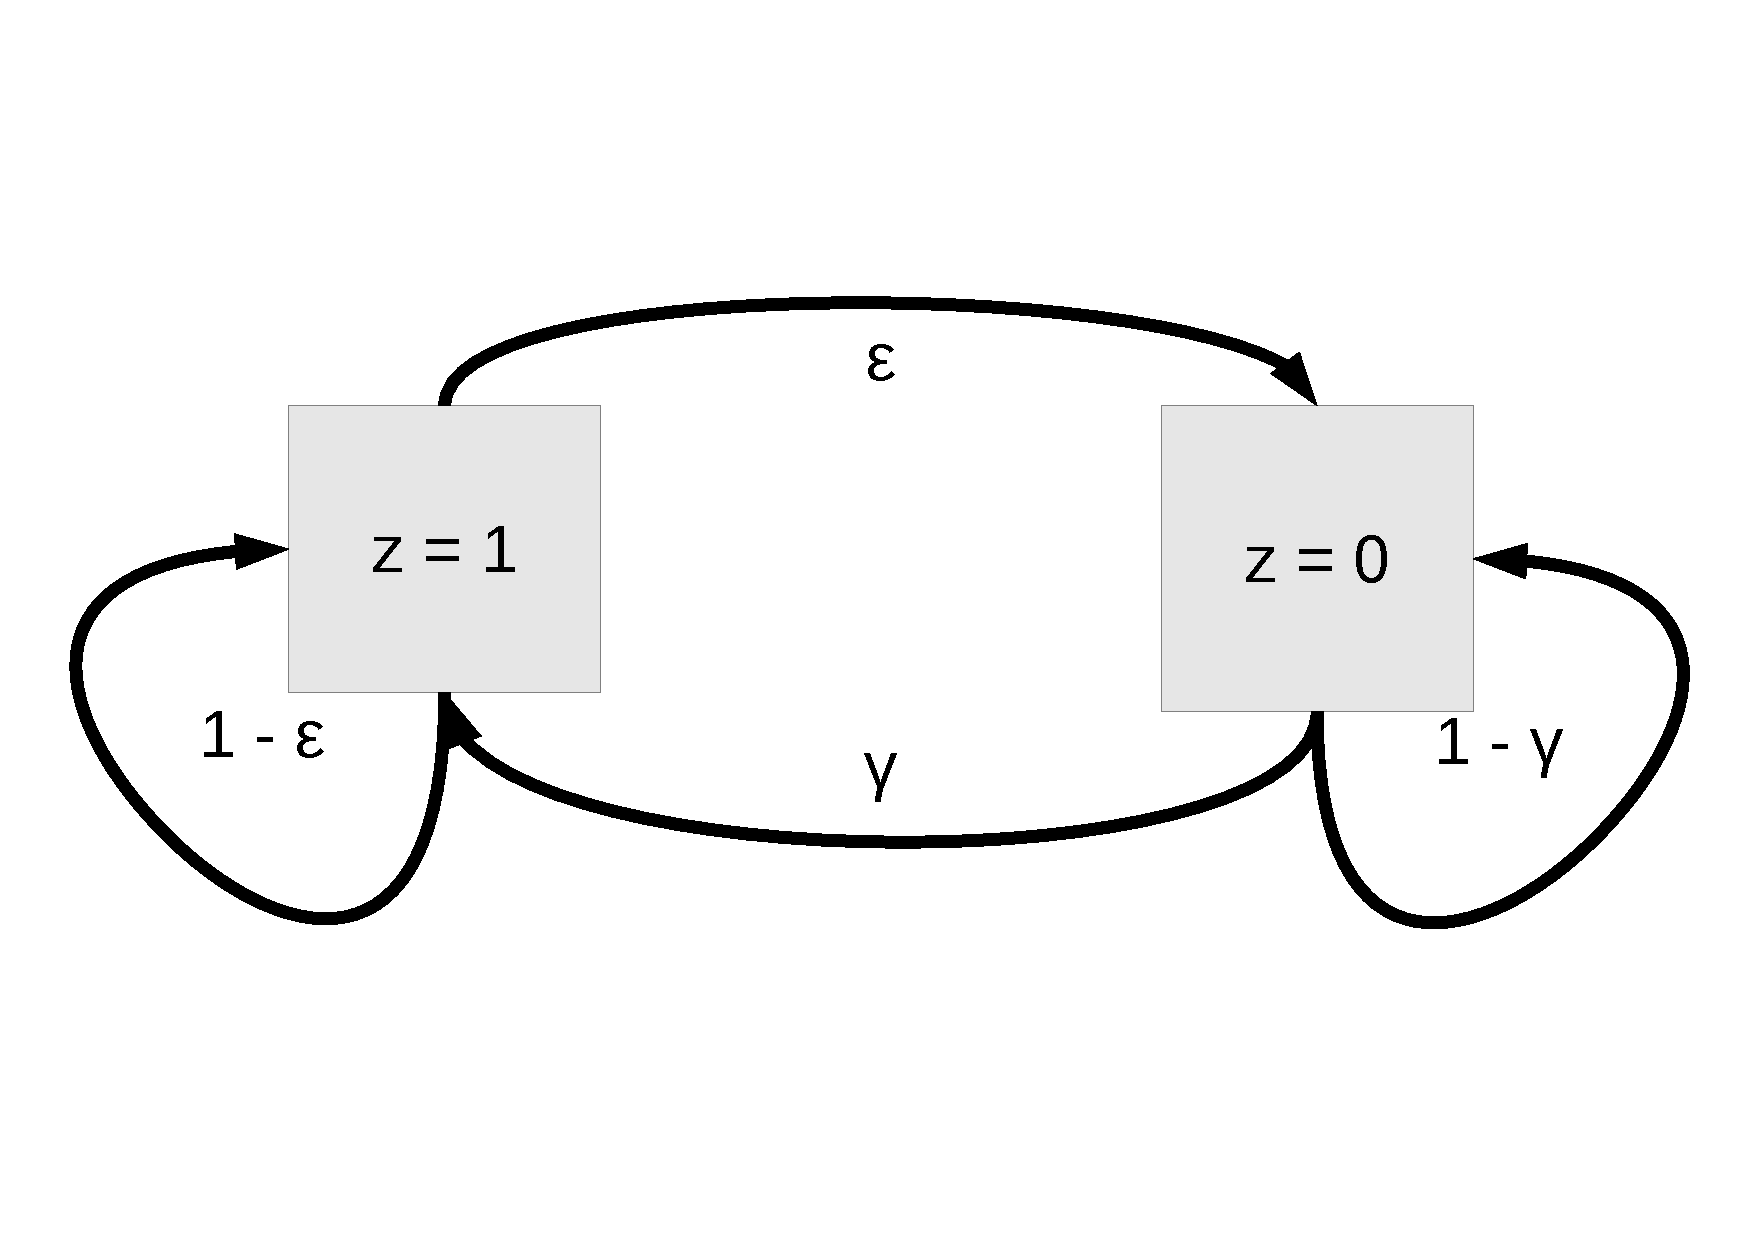
\includegraphics[width=\textwidth,height=0.8\textheight,keepaspectratio=true]{figure/mm_diagram}
  \end{center}
\end{frame}

\begin{frame}
  \frametitle{Model structure: hidden state}
  \begin{center}
    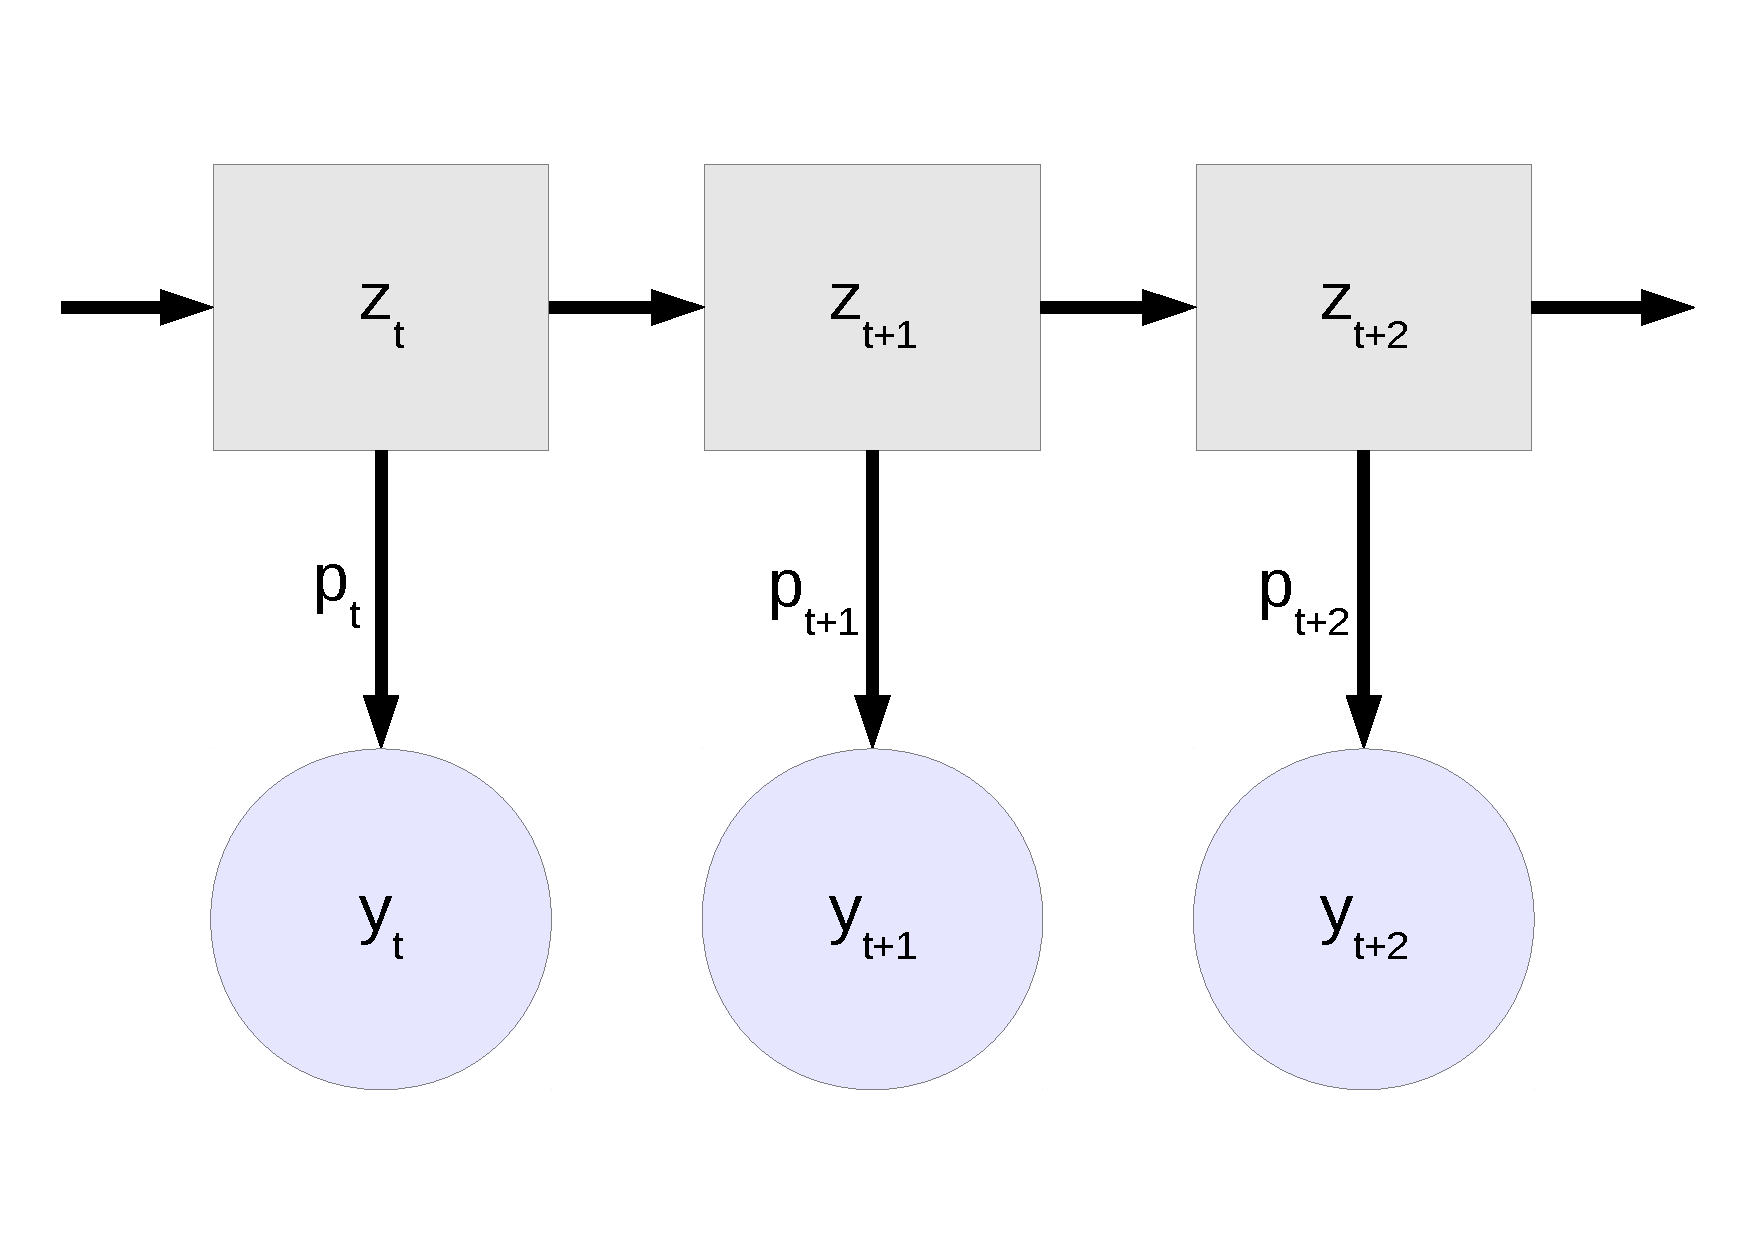
\includegraphics[width=\textwidth,height=0.8\textheight,keepaspectratio=true]{figure/hidden_state}
  \end{center}
\end{frame}


\begin{frame}
  \frametitle{Preliminary results}
\end{frame}

\begin{frame}
  \begin{block}{Major assumptions}
    \begin{itemize}
      \item model is only a first-order Markov process
        \begin{itemize}
          \item can lead to some taxa existing longer than in actuality
        \end{itemize}
      \item any taxon can occur in any geographic unit \\independent of other units
      \item both possibly controlled for by sampling rate through time
        \begin{itemize}
          \item further assumes all times and places can be considered similar
        \end{itemize}
      \item relaxing all of these assumption increases complexity
    \end{itemize}
  \end{block}
\end{frame}

\subsection{Mammals}
\begin{frame}
  \frametitle{Changes in Cenozoic mammal ecotype composition}

  \begin{alertblock}{Question}
    How do occurrence ratios of mammalian ecotypes change over time?
  \end{alertblock}
\end{frame}

\begin{frame}
  \frametitle{Environmental shift}
  % increasing aridity over cenozoic
  %   closed/forested --> open/grasslands
  %   sudden or slow?
  %     see Stromberg work
  \begin{center}
    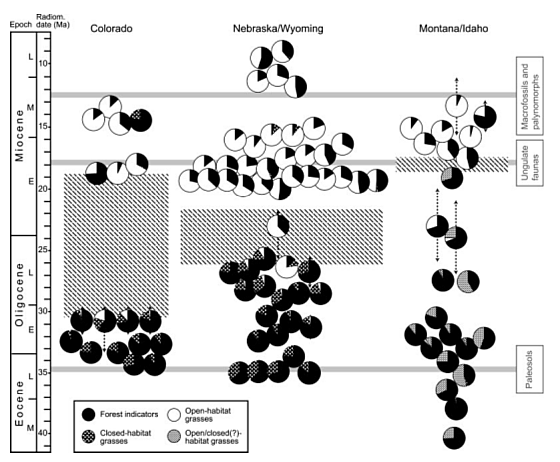
\includegraphics[width=\textwidth,height=0.8\textheight,keepaspectratio=true]{figure/stromberg_na}
  \end{center}

  \attrib{\small{Stromberg 2005 \emph{PNAS}}}
  % Smits2015 implies that increases in ``specialists'' would be due to speciation
\end{frame}

  % Janis reviews (annual reviews 1993)
  %   Eocene decrease in arboreal (and frugivorous)
  %   Eocene --> tropical forest
  %   Oligocene --> no analogy with modern
  %     greater proportion carnivores
  %     taxa are not typical of their clades (e.g. smaller)
  %       reason to use body size as predictor?
  %   Miocene --> savanna woodlands
  %     decrease in carnivores

\begin{frame}
  \frametitle{Possible link?}
  \begin{columns}
    \begin{column}{0.55\textwidth}
      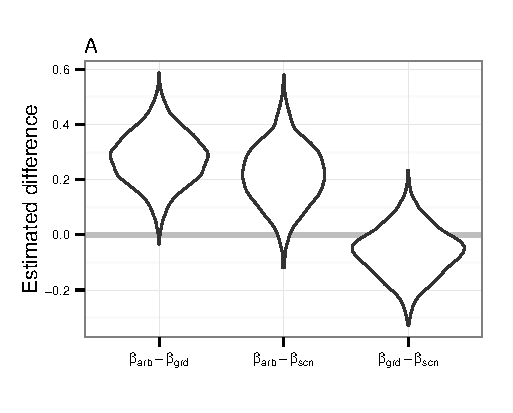
\includegraphics[width=\textwidth,height=0.8\textheight,keepaspectratio=true]{figure/loco_diff_est}
    \end{column}
    \begin{column}{0.55\textwidth}
      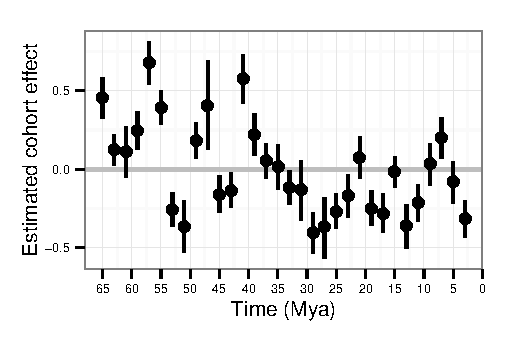
\includegraphics[width=\textwidth,height=\textheight,keepaspectratio=true]{figure/cohort_est}
    \end{column}
  \end{columns}

  \attrib{\small{Smits 2015 \emph{PNAS}}}
\end{frame}

\begin{frame}
  \frametitle{Multi-logit regression}
  \begin{equation*}
    \begin{aligned}
      y_{i} &\sim \mathrm{Categorical}(K, \pi) \\
      \pi_{k} &= \frac{\exp(\beta_{k, j[i]} X_{i} + \lambda_{k})}{\sum_{k = 1}^{K} \exp(\beta_{k, j[i]} X_{i} + \lambda_{k, i})} \\ 
      &\text{ where } \beta_{K, j[i]} X_{i} + \lambda_{K, i} = 0 \\
      \lambda_{k} &\sim \mathrm{MVN}(0, \tau_{k}^{2}\Sigma) \\
      \beta_{k, j} &\sim \mathcal{N}(\beta_{k}^{\prime}, \sigma_{k}) \\
    \end{aligned}
  \end{equation*}
\end{frame}

\begin{frame}
  \frametitle{Preliminary results}
\end{frame}

\begin{frame}
  \begin{block}{Further developments}
    \begin{itemize}
      \item \uppercase{\alert{note}} currently single flat mean; allow trend/multiple?
        \begin{itemize}
          \item time order is not currently modeled; all times exchangable
        \end{itemize}
      \item \uppercase{\alert{note}} technically no phylogenetic effect for \(k = K\)
      \item increased categorization (e.g. frugivory)?
      \item covariates (e.g. body size)?
      \item observed taxa represent a proportional sample of reality
        \begin{itemize}
          \item how can this be overcome in a \alert{model based} framework?
        \end{itemize}
      \item improve ``phylogeny''; I should do better than Smits 2015.
    \end{itemize}
  \end{block}
\end{frame}
  % coarseness of categories (no browse/graze difference)
  % no co-occurrence information
  %   lots of discussion on changes in beta diversity over Cenozoic
  %   makes things even more complicated
  %   a different study? was originally an idea, but needed better methods
  % slow; already slow with only 10% of the data
  %   three(!) phylogenetic effects
  % model improvement
  %   change point detection


\section{Timeline}
\begin{frame}
  \begin{block}{Things to consider}
    \begin{itemize}
      \item TAing this spring and next year
      \item Funding?
        \begin{itemize}
          \item FMNH fellow (but I don't spend time at the museum).
        \end{itemize}
      \item Estimates for time of completion?
      \item Post-doctoral opportunities?
    \end{itemize}
  \end{block}
\end{frame}

\begin{frame}
  \frametitle{Timeline}
  % timeline (finish next year plan)
  %   Winter quarter 2016
  %     next steps for current projects? (discussed previously)
  %       brachiopods
  %       mammals
  %   Spring quarter 2016
  %     TA: 
  %       hopefully Dimitry Kondrashov's Biological Modeling class
  %       otherwise i'd have to try and snag something in Greg and Stefano's new E&E class
  %     Evolution (June 17-21 Austin Texas):
  %       present something???
  %       meet people to talk post-doc opportunities (who???)
  %     Committee meeting:
  %       what are the goals between now and then?
  %       what should i have written (and sent to MORE people than just ken or michael)?
  %   Summer quarter 2016
  %   Fall quarter 2016
  %     GSA September 25-28 Denver Colorado
  %     SVP??? October 26-29 Salt Lace City Utah
  %     Committee meeting:
  %       what are the goals between now and then?
  %   Winter quarter 2017
  %   Spring quarter 2017
  %   Summer quarter 2017
\end{frame}




\end{document}
